\documentclass[12pt,a4paper]{article}
\usepackage[utf8]{inputenc}
\usepackage[margin=1in]{geometry}
\usepackage{graphicx}
\usepackage[hidelinks]{hyperref}
\usepackage{listings}
\usepackage{xcolor}
\usepackage{enumitem}
\usepackage{float}
\usepackage{tocloft}  % For customizing table of contents
% Define colors for syntax highlighting
\definecolor{codegreen}{rgb}{0,0.6,0}
\definecolor{codegray}{rgb}{0.5,0.5,0.5}
\definecolor{codepurple}{rgb}{0.58,0,0.82}
\definecolor{backcolour}{rgb}{0.95,0.95,0.92}

% Configure listing style for assembly code
\lstdefinestyle{mystyle}{
    backgroundcolor=\color{backcolour},
    commentstyle=\color{codegreen},
    keywordstyle=\color{blue},
    numberstyle=\tiny\color{codegray},
    stringstyle=\color{codepurple},
    basicstyle=\ttfamily\footnotesize,
    breakatwhitespace=false,
    breaklines=true,
    captionpos=b,
    keepspaces=true,
    numbers=left,
    numbersep=5pt,
    showspaces=false,
    showstringspaces=false,
    showtabs=false,
    tabsize=2
}

\lstset{style=mystyle}

\begin{document}
\begin{titlepage}
    \centering
    
    \vspace*{1cm}
    {\fontsize{20}{24}\bfseries University of Dhaka}\\[0.4cm]
    {\large Department of Computer Science and Engineering}\\[1cm]
    
    \hline
    \vspace{.5cm}
    {\Large \textbf{CSE 3113: Microprocessor and Assembly Lab}\\[.5cm]}
    
    \Large{Report of Tasks from Lab 2}
    \vspace{.5cm}
    \hline
    
    \vspace{1.5cm}
    
    % {\large \textbf{Lab Group: 03}}\\[0.5cm]
    
    \begin{center}
        \textbf{Submitted By} \\
        Muhaiminul Islam Ninad \\
        Roll:  43
    \end{center}
    
    
    \vspace{1.5cm}
    
    {\large \textbf{Submitted To:}}\\[0.4cm]
    Dr. Upama Kabir \\
    Professor,  Dept. of CSE, University of Dhaka\\[.3cm]
    Dr. Mosarrat Jahan \\
    Associate Professor, Dept. of CSE, University of Dhaka \\[.3cm]
    Mr. Jargis Ahmed, \\
    Lecturer, Dept. of CSE, University of Dhaka\\[.3cm]
    Mr. Palash Roy, \\
    Lecturer, Dept. of CSE, University of Dhaka\\[1.3cm]
    
    {\large \textbf{Submission Date:} \today}
    
    \vfill
    
\end{titlepage}

\tableofcontents
\newpage

\section{Task 1: Addition of Two 16-bit Variables}

\subsection{Code with Comments}
The following assembly code adds the contents of the 16-bit variable X to the contents of the 16-bit variable Y and places the result in the 16-bit variable Result:

\begin{lstlisting}[language={}]
    AREA STACK, NOINIT, READWRITE, ALIGN=3
    SPACE 1024                  ; Reserve 1024 bytes for stack
    
    AREA |.vectors|, CODE, READONLY
    EXPORT __Vectors
__Vectors
    DCD __stack_top             ; Initial stack pointer
    DCD Reset_Handler           ; Reset handler
    DCD 0                       ; NMI handler (placeholder)
    DCD 0                       ; HardFault handler (placeholder)
    
    AREA |startup|, CODE, READONLY
__stack_top EQU STACK + 1024
    EXPORT Reset_Handler
Reset_Handler
    BL main                     ; Call main
    B .                         ; Loop forever if main returns
    
    AREA |.data|, DATA, READWRITE
X       DCW 0x1234              ; Define 16-bit value for X
Y       DCW 0x4321              ; Define 16-bit value for Y
Result  DCW 0x0001              ; Result placeholder
    
    AREA |.text|, CODE, READONLY
main
    LDR r0, =X                  ; Load address of X
    LDRH r1, [r0]               ; Load value of X into r1
    
    LDR r0, =Y                  ; Load address of Y
    LDRH r2, [r0]               ; Load value of Y into r2
    
    ADD r3, r1, r2              ; Add X and Y, store result in r3
    
    LDR r0, =Result             ; Load address of Result
    STRH r3, [r0]               ; Store result in memory
STOP
    B STOP                      ; Infinite loop
    END
\end{lstlisting}

\subsection{Code Explanation}
The assembly code can be broken down into several key components:

\subsubsection{Memory and Stack Setup}
\begin{itemize}
    \item \texttt{AREA STACK} directive allocates 1024 bytes for the stack
    \item Vector table defines essential handlers including the reset handler
\end{itemize}

\subsubsection{Data Section}
\begin{itemize}
    \item Variables X and Y are defined as 16-bit values (0x1234 and 0x4321)
    \item Result is initialized with a placeholder value
\end{itemize}

\subsubsection{Main Logic}
\begin{itemize}
    \item The address of X is loaded into register r0
    \item The 16-bit value of X is loaded into register r1 using LDRH (Load Register Halfword)
    \item The address of Y is loaded into register r0
    \item The 16-bit value of Y is loaded into register r2 using LDRH
    \item The ADD instruction adds r1 and r2, storing the result in r3
    \item The address of Result is loaded into register r0
    \item The STRH (Store Register Halfword) instruction stores the 16-bit value in r3 to the Result variable
\end{itemize}

\subsubsection{Expected Results}
Adding 0x1234 (4660 in decimal) to 0x4321 (17185 in decimal) yields 0x5555 (21845 in decimal), which will be stored in the Result variable.

\subsection{System State Screenshots}
\subsubsection{System State After Code Loading}
\begin{figure}[H]
    \centering
    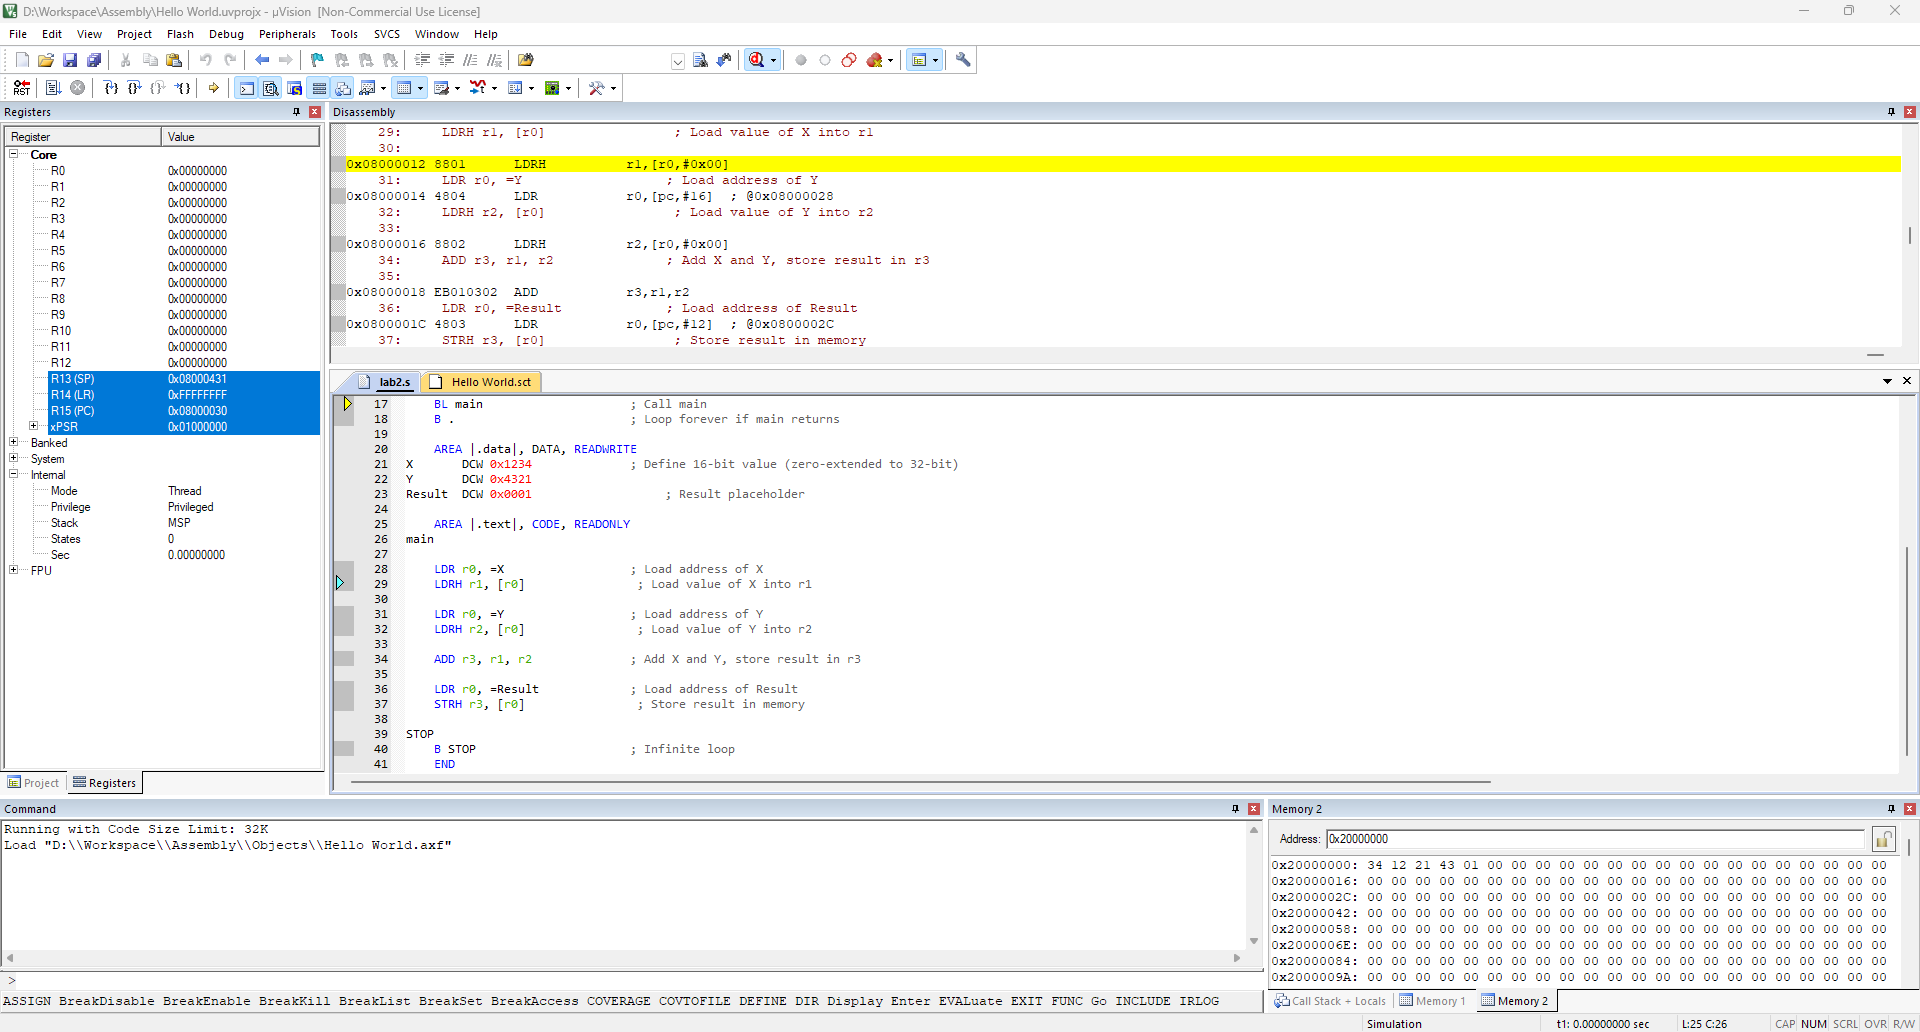
\includegraphics[width=\textwidth]{ls1.png}
    \caption{Memory contents after loading the assembly code}
    \label{fig:loading1}
\end{figure}

\subsubsection{System State After Code Execution}
\begin{figure}[H]
    \centering
    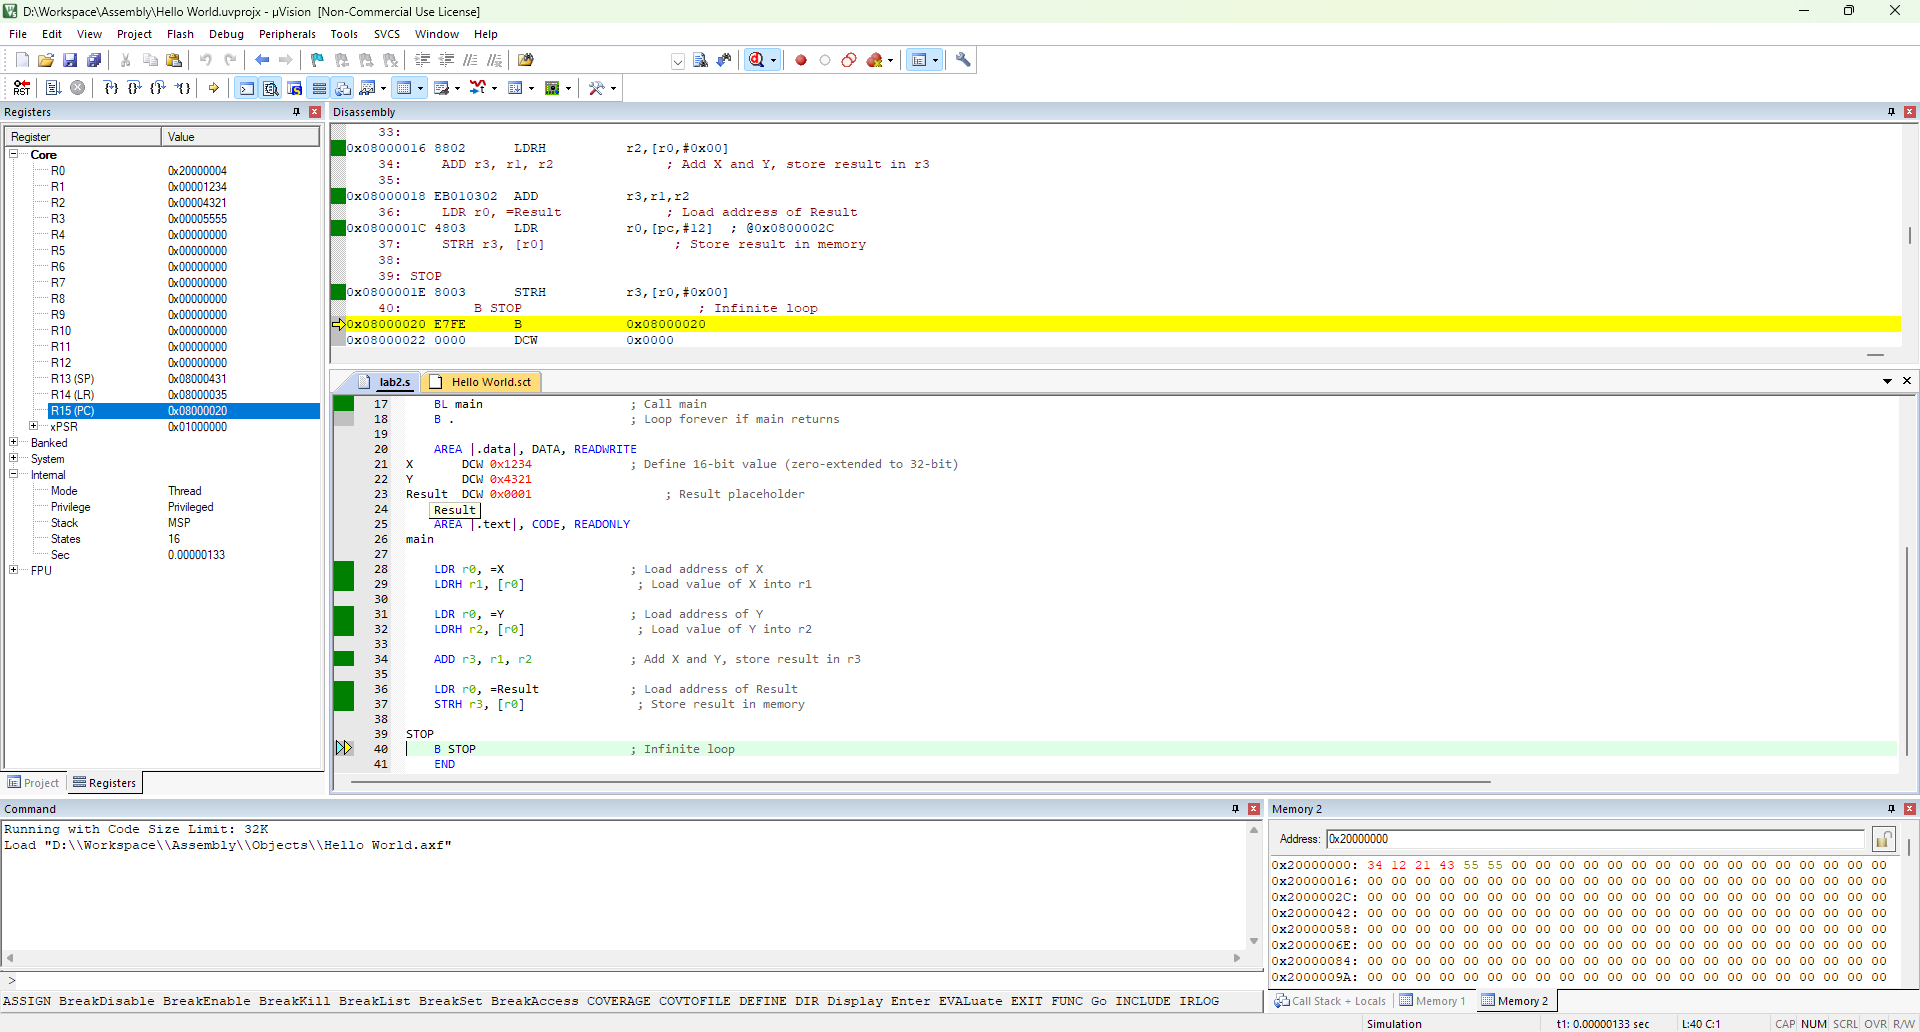
\includegraphics[width=\textwidth]{es1.png}
    \caption{Memory contents after executing the assembly code}
    \label{fig:execution1}
\end{figure}

\section{Task 2: Arithmetic Operations on Two Variables}

\subsection{Code with Comments}
The following assembly code performs addition, subtraction, and multiplication on two 16-bit variables X and Y:

\begin{lstlisting}[language={}]
    AREA STACK, NOINIT, READWRITE, ALIGN=3
    SPACE 1024                  ; Reserve 1024 bytes for stack

    AREA |.vectors|, CODE, READONLY
    EXPORT __Vectors
__Vectors
    DCD __stack_top             ; Initial stack pointer
    DCD Reset_Handler           ; Reset handler
    DCD 0                       ; NMI handler (placeholder)
    DCD 0                       ; HardFault handler (placeholder)

    AREA |startup|, CODE, READONLY
__stack_top EQU STACK + 1024

    EXPORT Reset_Handler
Reset_Handler
    BL main                     ; Call main
    B .                         ; Loop forever if main returns

    AREA |.data|, DATA, READWRITE
X           DCW 0x4321          ; Define 16-bit value
Y           DCW 0x1234          ; Define another 16-bit value
Result_Add  DCW 0x0000          ; Placeholder for Addition result
Result_Sub  DCW 0x0000          ; Placeholder for Subtraction result
Result_Mul  DCD 0x0000          ; Placeholder for Multiplication result

    AREA |.text|, CODE, READONLY
main
    ; Load X into r1
    LDR r0, =X
    LDRH r1, [r0]

    ; Load Y into r2
    LDR r0, =Y
    LDRH r2, [r0]

    ; -------- Addition --------
    ADD r3, r1, r2              ; r3 = r1 + r2
    LDR r0, =Result_Add
    STRH r3, [r0]

    ; -------- Subtraction --------
    SUB r3, r1, r2              ; r3 = r1 - r2
    LDR r0, =Result_Sub
    STRH r3, [r0]

    ; -------- Multiplication --------
    MUL r3, r1, r2              ; r3 = r1 * r2
    LDR r0, =Result_Mul
    STR r3, [r0]                ; Store full 32 bits (since multiplication can overflow 16 bits)
	

STOP
    B STOP                      ; Infinite loop
    END
\end{lstlisting}

\subsection{Code Explanation}
This code extends the previous example to include three arithmetic operations:

\subsubsection{Data Section}
\begin{itemize}
    \item X is defined as 0x4321 (17185 in decimal)
    \item Y is defined as 0x1234 (4660 in decimal)
    \item Three result variables are defined for different operations
\end{itemize}

\subsubsection{Main Logic}
\begin{itemize}
    \item Values of X and Y are loaded into registers r1 and r2 respectively
    \item Addition: r1 + r2 stored in r3, then stored in the Addition variable
    \item Subtraction: r1 - r2 stored in r3, then stored in the Subtraction variable
    \item Multiplication: r1 * r2 stored in r3, then stored in the Multiplication variable
\end{itemize}

\subsubsection{Expected Results}
\begin{itemize}
    \item Addition: 0x4321 + 0x1234 = 0x5555 (17185 + 4660 = 21845)
    \item Subtraction: 0x4321 - 0x1234 = 0x30ED (17185 - 4660 = 12525)
    \item Multiplication: 0x4321 * 0x1234 = 0x4ECA564 (17185 * 4660 = 80,082,100)
        \begin{itemize}
            \item Note: The multiplication result requires 32 bits to store properly, which is why we use STR instead of STRH for the result.
        \end{itemize}
\end{itemize}

\subsection{System State Screenshots}
\subsubsection{System State After Code Loading}
\begin{figure}[H]
    \centering
    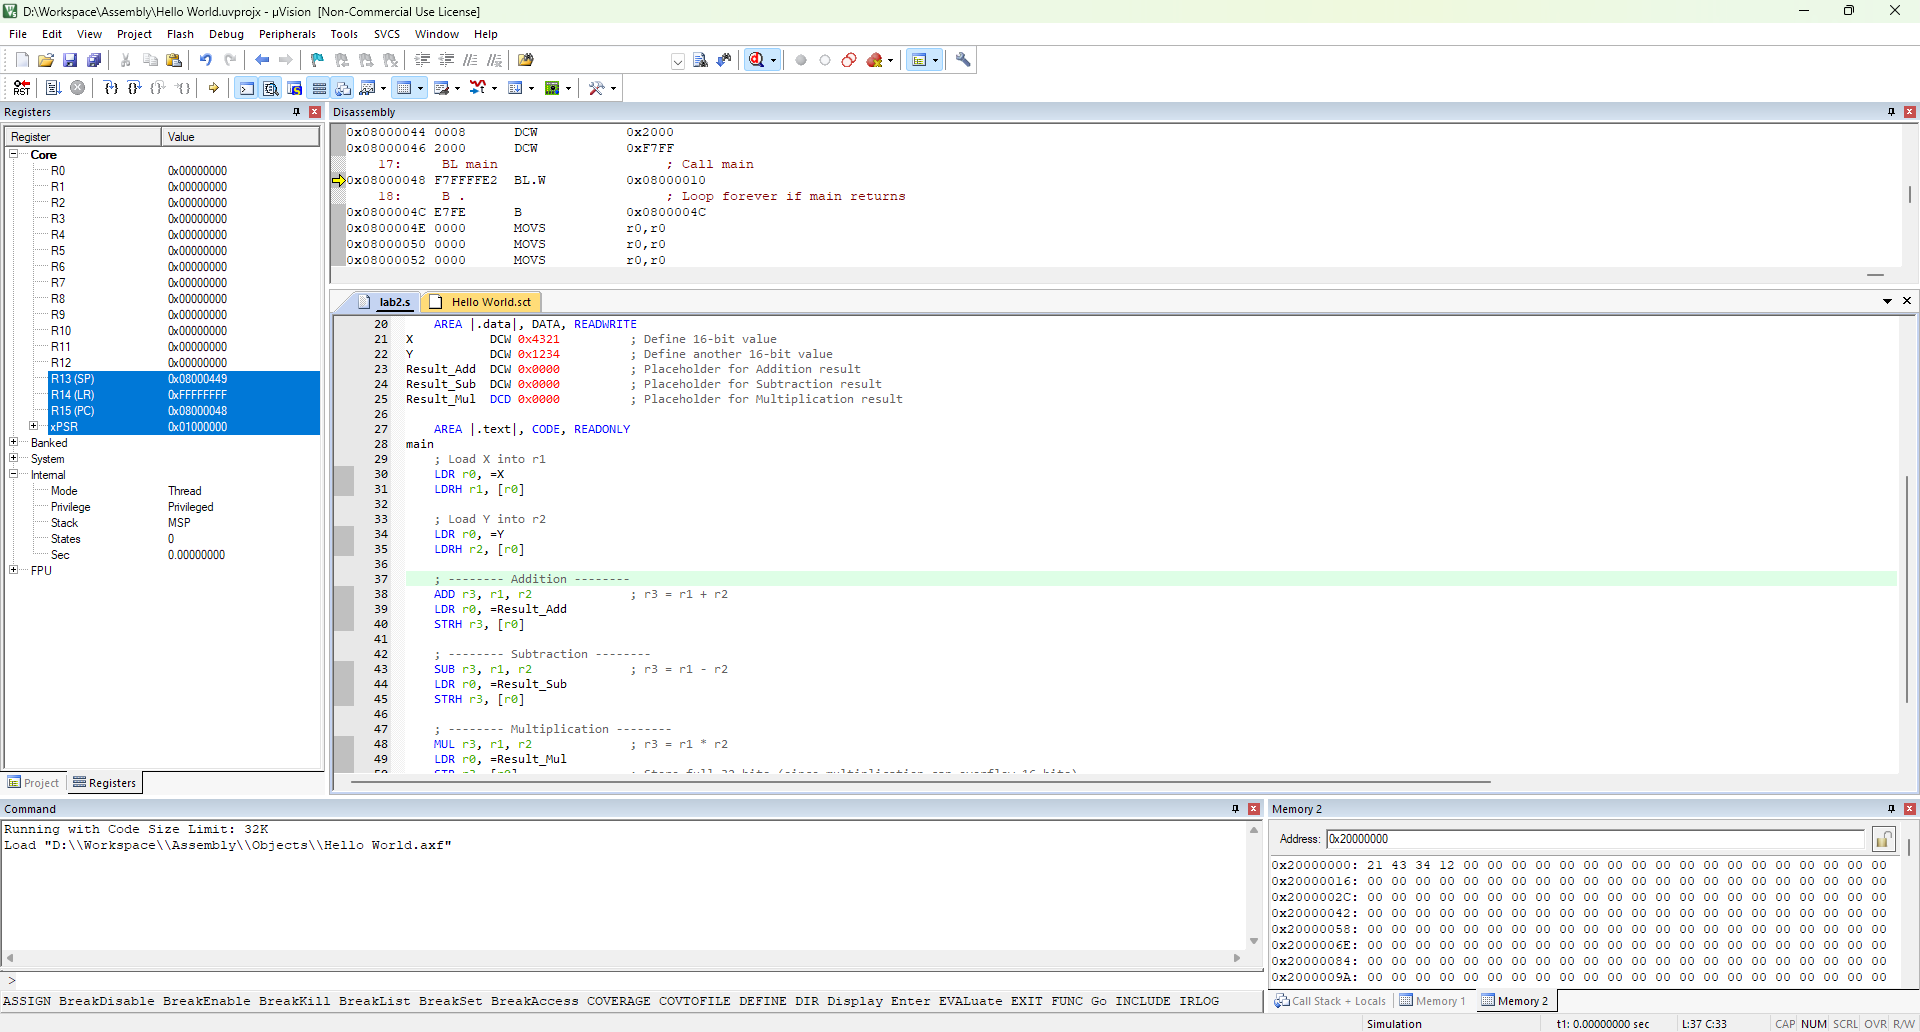
\includegraphics[width=\textwidth]{ls2.png}
    \caption{Memory contents after loading the assembly code}
    \label{fig:loading2}
\end{figure}

\subsubsection{System State After Code Execution}
\begin{figure}[H]
    \centering
    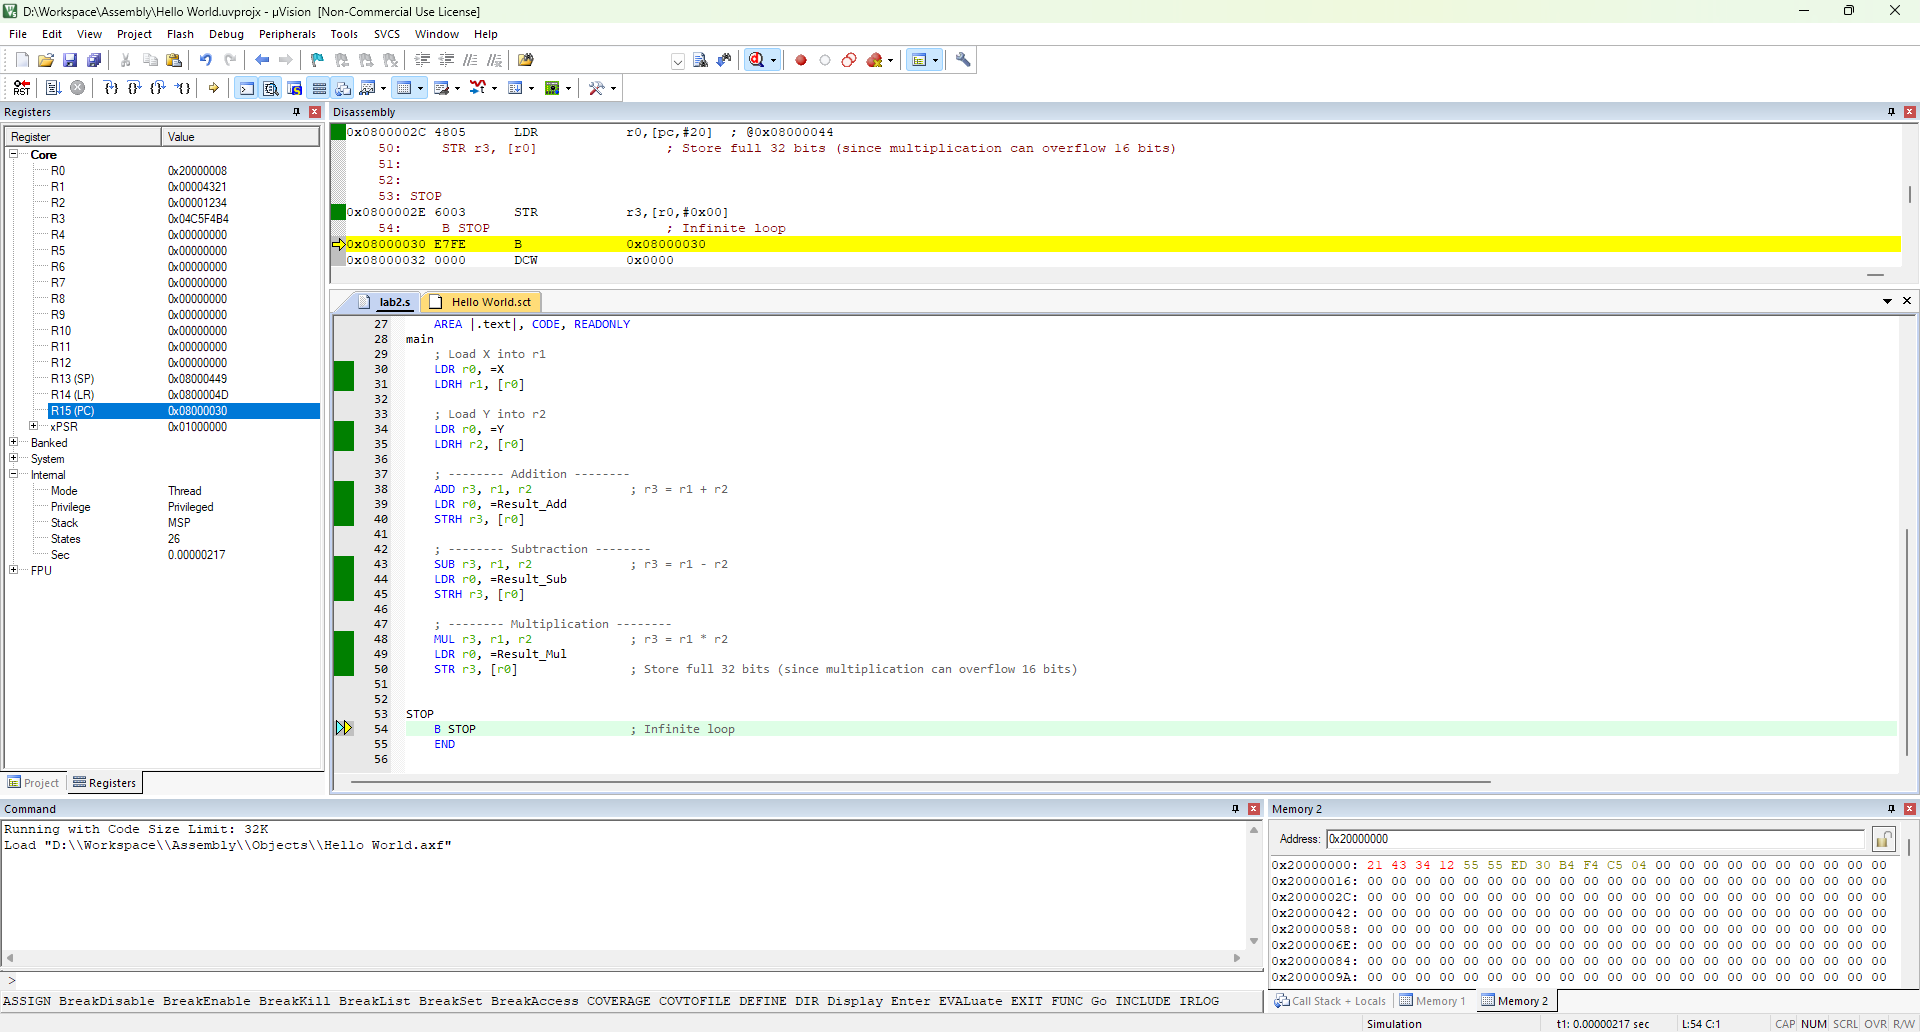
\includegraphics[width=\textwidth]{es2.png}
    \caption{Memory contents after executing the assembly code}
    \label{fig:execution2}
\end{figure}

\section{Task 3: Finding the Smaller of Two Integer Numbers}

\subsection{Code with Comments}
The following assembly code finds the smaller of two integer numbers:

\begin{lstlisting}[language={}]
    AREA STACK, NOINIT, READWRITE, ALIGN=3
    SPACE 1024                  ; Reserve 1024 bytes for stack
    
    AREA |.vectors|, CODE, READONLY
    EXPORT __Vectors
__Vectors
    DCD __stack_top             ; Initial stack pointer
    DCD Reset_Handler           ; Reset handler
    DCD 0                       ; NMI handler (placeholder)
    DCD 0                       ; HardFault handler (placeholder)
    
    AREA |startup|, CODE, READONLY
__stack_top EQU STACK + 1024
    EXPORT Reset_Handler
Reset_Handler
    BL main                     ; Call main
    B .                         ; Loop forever if main returns
    
    AREA |.data|, DATA, READWRITE
Num1        DCW 0x0018          ; First number (24 in decimal)
Num2        DCW 0x002A          ; Second number (42 in decimal)
SmallerNum  DCW 0x0000          ; Will store the smaller number
    
    AREA |.text|, CODE, READONLY
main
    ; Load the values of Num1 and Num2
    LDR r0, =Num1               ; Load address of Num1
    LDRH r1, [r0]               ; Load value of Num1 into r1
    
    LDR r0, =Num2               ; Load address of Num2
    LDRH r2, [r0]               ; Load value of Num2 into r2
    
    ; Compare the two numbers
    CMP r1, r2                  ; Compare r1 (Num1) with r2 (Num2)
    BLS Num1IsSmaller           ; Branch if r1 <= r2 (Num1 is smaller or equal)
    
    ; If we get here, Num2 is smaller
    LDR r0, =SmallerNum         ; Load address of SmallerNum
    STRH r2, [r0]               ; Store Num2 as the smaller number
    B Done                      ; Branch to Done
    
Num1IsSmaller
    LDR r0, =SmallerNum         ; Load address of SmallerNum
    STRH r1, [r0]               ; Store Num1 as the smaller number
    
Done
STOP
    B STOP                      ; Infinite loop
    END
\end{lstlisting}

\subsection{Code Explanation}
This code compares two numbers and finds the smaller one:

\subsubsection{Data Section}
\begin{itemize}
    \item Num1 is defined as 0x0018 (24 in decimal)
    \item Num2 is defined as 0x002A (42 in decimal)
    \item SmallerNum is initialized to store the result
\end{itemize}

\subsubsection{Main Logic}
\begin{itemize}
    \item Values of Num1 and Num2 are loaded into registers r1 and r2 respectively
    \item CMP instruction compares r1 and r2
    \item BLS (Branch if Lower or Same) instruction checks if r1 $\leq$ r2
    \item If r1 $\leq$ r2, the code branches to Num1IsSmaller
    \item Otherwise, r2 is assumed to be smaller and stored in SmallerNum
    \item At Num1IsSmaller, r1 is stored in SmallerNum
\end{itemize}

\subsubsection{Expected Results}
Since Num1 (24) is smaller than Num2 (42), the value 0x0018 (24) will be stored in SmallerNum.

\subsection{System State Screenshots}
\subsubsection{System State After Code Loading}
\begin{figure}[H]
    \centering
    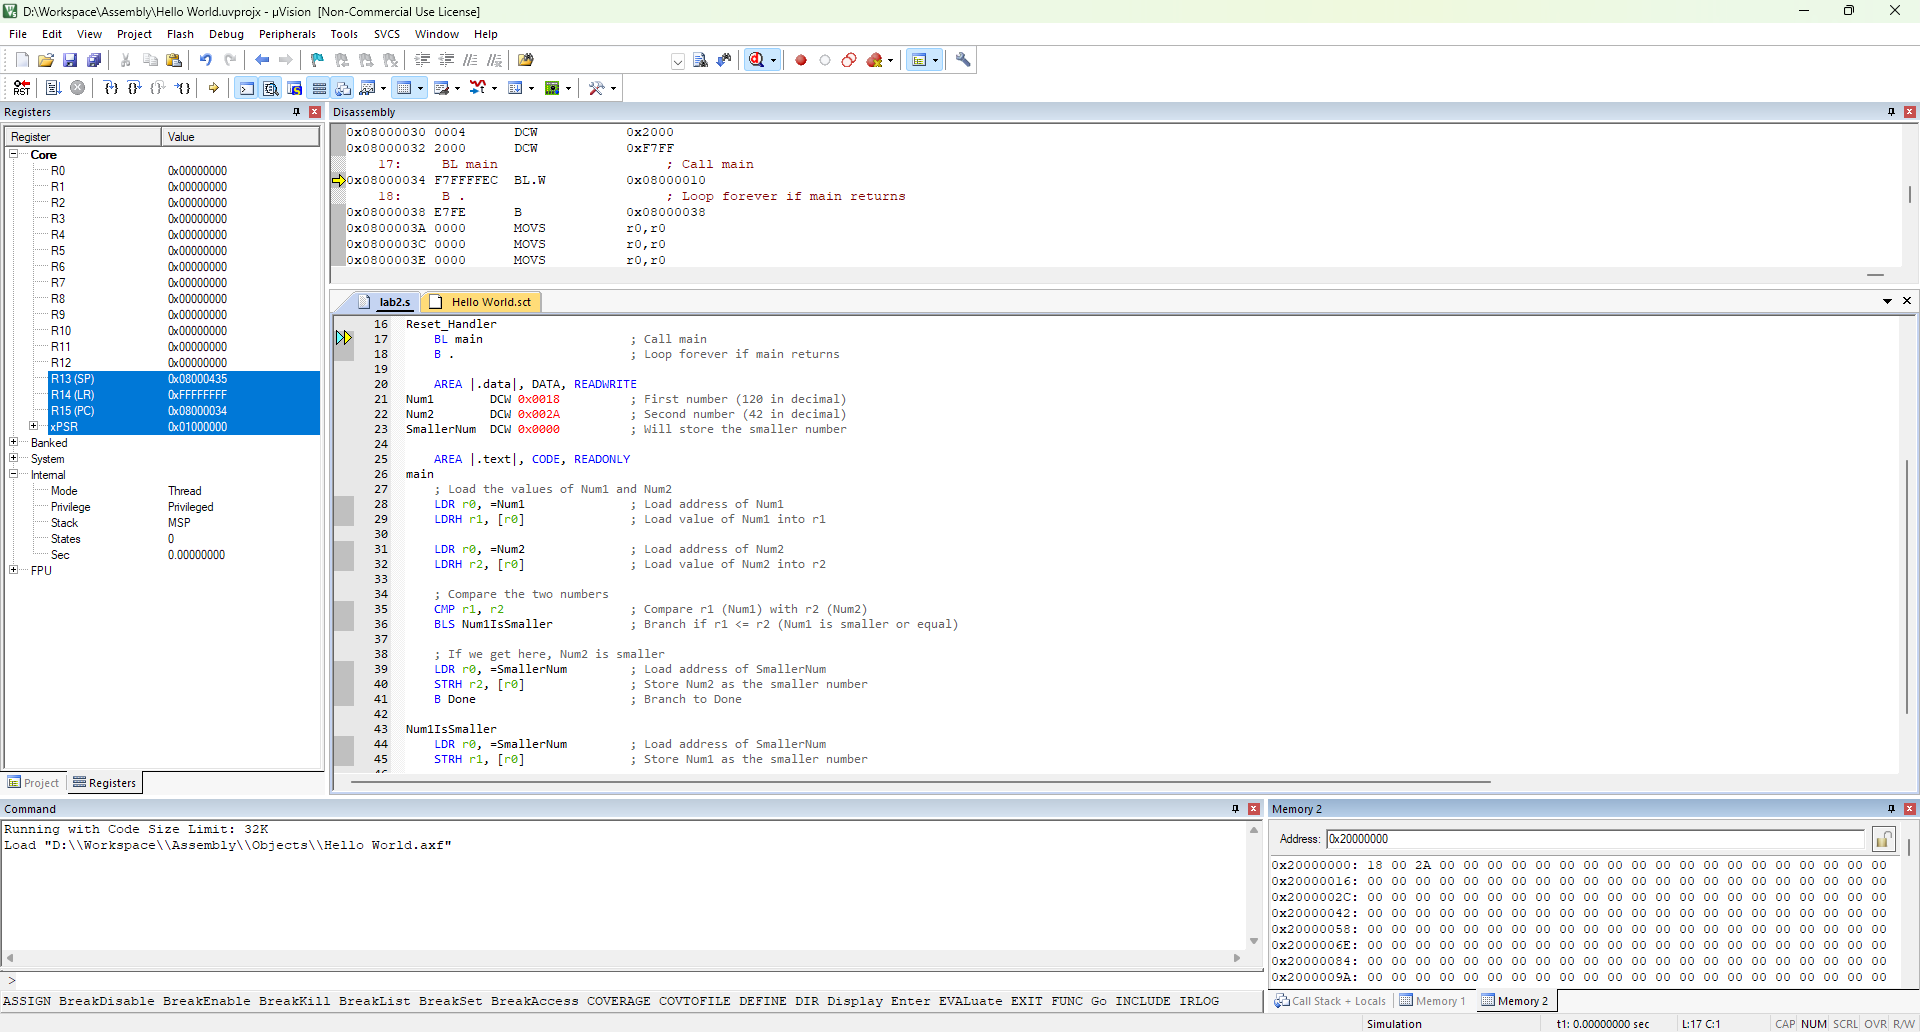
\includegraphics[width=\textwidth]{ls3.png}
    \caption{Memory contents after loading the assembly code}
    \label{fig:loading3}
\end{figure}

\subsubsection{System State After Code Execution}
\begin{figure}[H]
    \centering
    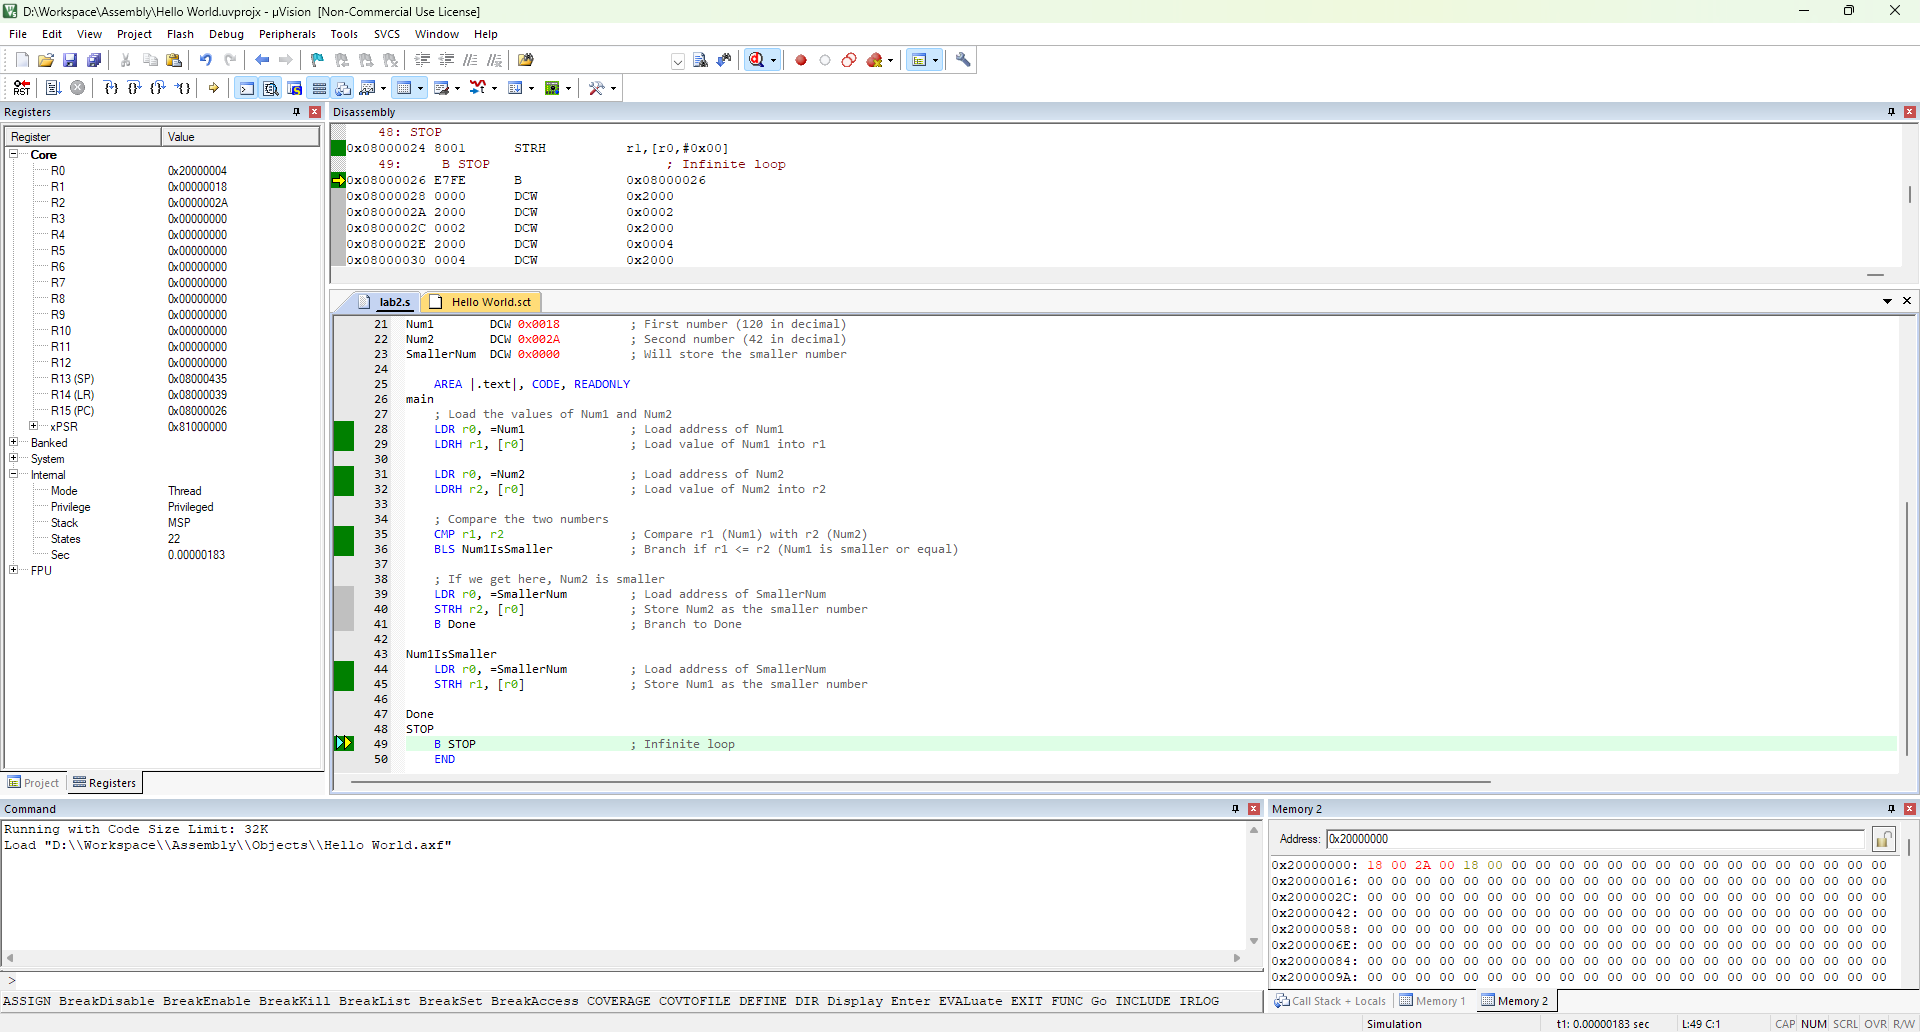
\includegraphics[width=\textwidth]{es3.png}
    \caption{Memory contents after executing the assembly code}
    \label{fig:execution3}
\end{figure}

\section{Conclusion}
This lab demonstrated the implementation of basic arithmetic operations and comparison logic in assembly language. The programs successfully:
\begin{itemize}
    \item Added two 16-bit variables
    \item Performed addition, subtraction, and multiplication on two variables
    \item Found the smaller of two integer numbers
\end{itemize}

These implementations illustrate fundamental assembly language concepts including memory access, register operations, and conditional branching.

\end{document}